% Options for packages loaded elsewhere
\PassOptionsToPackage{unicode}{hyperref}
\PassOptionsToPackage{hyphens}{url}
\PassOptionsToPackage{dvipsnames,svgnames,x11names}{xcolor}
%
\documentclass[
  12pt,
]{article}
\usepackage{amsmath,amssymb}
\usepackage{iftex}
\ifPDFTeX
  \usepackage[T1]{fontenc}
  \usepackage[utf8]{inputenc}
  \usepackage{textcomp} % provide euro and other symbols
\else % if luatex or xetex
  \usepackage{unicode-math} % this also loads fontspec
  \defaultfontfeatures{Scale=MatchLowercase}
  \defaultfontfeatures[\rmfamily]{Ligatures=TeX,Scale=1}
\fi
\usepackage{lmodern}
\ifPDFTeX\else
  % xetex/luatex font selection
\fi
% Use upquote if available, for straight quotes in verbatim environments
\IfFileExists{upquote.sty}{\usepackage{upquote}}{}
\IfFileExists{microtype.sty}{% use microtype if available
  \usepackage[]{microtype}
  \UseMicrotypeSet[protrusion]{basicmath} % disable protrusion for tt fonts
}{}
\makeatletter
\@ifundefined{KOMAClassName}{% if non-KOMA class
  \IfFileExists{parskip.sty}{%
    \usepackage{parskip}
  }{% else
    \setlength{\parindent}{0pt}
    \setlength{\parskip}{6pt plus 2pt minus 1pt}}
}{% if KOMA class
  \KOMAoptions{parskip=half}}
\makeatother
\usepackage{xcolor}
\usepackage[margin=1in]{geometry}
\usepackage{graphicx}
\makeatletter
\def\maxwidth{\ifdim\Gin@nat@width>\linewidth\linewidth\else\Gin@nat@width\fi}
\def\maxheight{\ifdim\Gin@nat@height>\textheight\textheight\else\Gin@nat@height\fi}
\makeatother
% Scale images if necessary, so that they will not overflow the page
% margins by default, and it is still possible to overwrite the defaults
% using explicit options in \includegraphics[width, height, ...]{}
\setkeys{Gin}{width=\maxwidth,height=\maxheight,keepaspectratio}
% Set default figure placement to htbp
\makeatletter
\def\fps@figure{htbp}
\makeatother
\setlength{\emergencystretch}{3em} % prevent overfull lines
\providecommand{\tightlist}{%
  \setlength{\itemsep}{0pt}\setlength{\parskip}{0pt}}
\setcounter{secnumdepth}{5}
\newlength{\cslhangindent}
\setlength{\cslhangindent}{1.5em}
\newlength{\csllabelwidth}
\setlength{\csllabelwidth}{3em}
\newlength{\cslentryspacingunit} % times entry-spacing
\setlength{\cslentryspacingunit}{\parskip}
\newenvironment{CSLReferences}[2] % #1 hanging-ident, #2 entry spacing
 {% don't indent paragraphs
  \setlength{\parindent}{0pt}
  % turn on hanging indent if param 1 is 1
  \ifodd #1
  \let\oldpar\par
  \def\par{\hangindent=\cslhangindent\oldpar}
  \fi
  % set entry spacing
  \setlength{\parskip}{#2\cslentryspacingunit}
 }%
 {}
\usepackage{calc}
\newcommand{\CSLBlock}[1]{#1\hfill\break}
\newcommand{\CSLLeftMargin}[1]{\parbox[t]{\csllabelwidth}{#1}}
\newcommand{\CSLRightInline}[1]{\parbox[t]{\linewidth - \csllabelwidth}{#1}\break}
\newcommand{\CSLIndent}[1]{\hspace{\cslhangindent}#1}
\ifLuaTeX
\usepackage[bidi=basic]{babel}
\else
\usepackage[bidi=default]{babel}
\fi
\babelprovide[main,import]{spanish}
% get rid of language-specific shorthands (see #6817):
\let\LanguageShortHands\languageshorthands
\def\languageshorthands#1{}
\usepackage{float}
\ifLuaTeX
  \usepackage{selnolig}  % disable illegal ligatures
\fi
\IfFileExists{bookmark.sty}{\usepackage{bookmark}}{\usepackage{hyperref}}
\IfFileExists{xurl.sty}{\usepackage{xurl}}{} % add URL line breaks if available
\urlstyle{same}
\hypersetup{
  pdftitle={Proyecto final - Egresos del Sector Público},
  pdfauthor={Ignacio Campón},
  pdflang={es},
  colorlinks=true,
  linkcolor={blue},
  filecolor={Maroon},
  citecolor={blue},
  urlcolor={blue},
  pdfcreator={LaTeX via pandoc}}

\title{Proyecto final - Egresos del Sector Público}
\usepackage{etoolbox}
\makeatletter
\providecommand{\subtitle}[1]{% add subtitle to \maketitle
  \apptocmd{\@title}{\par {\large #1 \par}}{}{}
}
\makeatother
\subtitle{Series Cronológicas, 2024}
\author{Ignacio Campón}
\date{}

\begin{document}
\maketitle

\maketitle

\thispagestyle{empty} % Hide header and footer on the title page
\vspace*{\fill} % Pushes content to the bottom of the page
\begin{center}

\includegraphics[width=16cm]{imagenes/logo_inst_80.png}\\[1cm] % Adjust image placement
\end{center}

\newpage

\hypertarget{resuxfamen-ejecutivo}{%
\section*{Resúmen Ejecutivo}\label{resuxfamen-ejecutivo}}
\addcontentsline{toc}{section}{Resúmen Ejecutivo}

Este trabajo busca el estudio de identificación, estimación y prediccón
de una serie de tiempo. Se analizan los \textbf{Egresos Primarios del
Sector Público no Monetario} en Uruguay, entre enero de 1999 y abril de
2024. La serie de tiempo mensual, proporcionada por el
\href{https://www.gub.uy/ministerio-economia-finanzas/datos-y-estadisticas/estadisticas/informacion-resultados-del-sector-publico}{Ministerio
de Economía y Finanzas}, es fundamental para comprender la dinámica
fiscal del país y anticipar tendencias futuras en base a modelos
estadísticos. Siguiendo la metodología de Box y Jenkins, se busca
identificar un modelo SARIMA a partir de la función de autocorrelación y
autocorrelación parcial. Los modelos propuesto son puestos a prueba a
través de una etapa de diagnostico obteniendo un modelo final con el
cual es realizada la predicción. Para esta se dividien los datos en
conjuntos de entrenamiento y prueba a efectos de validar el modelo.

\newpage

\tableofcontents

\newpage

\hypertarget{introducciuxf3n}{%
\section{Introducción}\label{introducciuxf3n}}

En el contexto del análisis económico y financiero, los \textbf{Egresos
Primarios del Sector Público no Monetario}, son una fuente crucial de
información proporcionada por el
\href{https://www.gub.uy/ministerio-economia-finanzas/datos-y-estadisticas/estadisticas/informacion-resultados-del-sector-publico}{Ministerio
de Economía y Finanzas}. Esta serie mensual, ofrece una panorámica
detallada de los desembolsos financieros del sector público, excluyendo
transacciones monetarias, a lo largo del tiempo.

Los egresos primarios del sector público son fundamentales para entender
la dinámica fiscal de un país, ya que representan los gastos esenciales
en bienes y servicios no financieros realizados por el gobierno. Estos
datos son vitales para analizar la gestión presupuestaria, evaluar
políticas económicas y anticipar tendencias futuras en base a modelos
estadísticos. En este informe, se explorará la serie temporal con el
objetivo de identificar un modelo adecuado que permita reproducirla con
precisión, facilitando así la capacidad predictiva sobre los egresos del
sector público en Uruguay.

\hypertarget{anuxe1lisis-exploratorio}{%
\subsection{Análisis Exploratorio}\label{anuxe1lisis-exploratorio}}

La serie de Egresos Primarios del Sector Público no Monetario, abarca el
período comprendido entre enero de 1999 y abril de 2024. Veáse la figura
\ref{gasto_publico}. A lo largo de los años, se observa un crecimiento
sostenido en los desembolsos del sector público, con fluctuaciones
estacionales y ciertas tendencias a lo largo del tiempo. La serie
presenta una tendencia creciente, con una estacionalidad marcada por
picos y valles en determinados puntos lo cual destaca una no
estacionariedad en la serie.

\begin{figure}[H]

{\centering 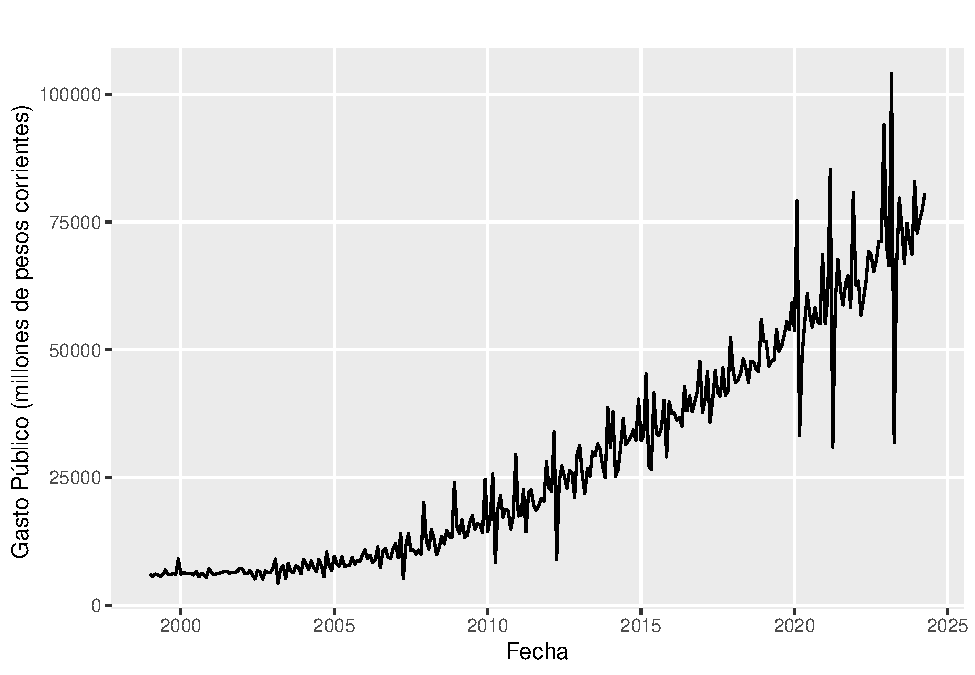
\includegraphics[width=0.75\linewidth]{informe_files/figure-latex/plot_series_inicial-1} 

}

\caption{\label{gasto_publico} Evolución del Gasto Público mensual en millones de pesos corrientes entre enero 1999 y abril 2024.}\label{fig:plot_series_inicial}
\end{figure}

Estos patrones sugieren la presencia de componentes estacionales. La
figura \ref{month_plot} muestra el comportamiento mensual del Gasto
Público entre 1999 y 2024. Se observa una clara estacionalidad en la
serie, los picos y valles que se ven en la figura \ref{gasto_publico},
han de corresponderse a los meses de diciembre y abril respectivamente.
La diferencia en las medias son notorias para los meses mencionados,
siendo los puntos donde se alcanza el máximo (diciembre) y mínimo
(abril) en promedio. Esto sugiere una estacionalidad anual, la cual será
un factor importante a considerar en el modelado de la serie.

\begin{figure}[H]

{\centering 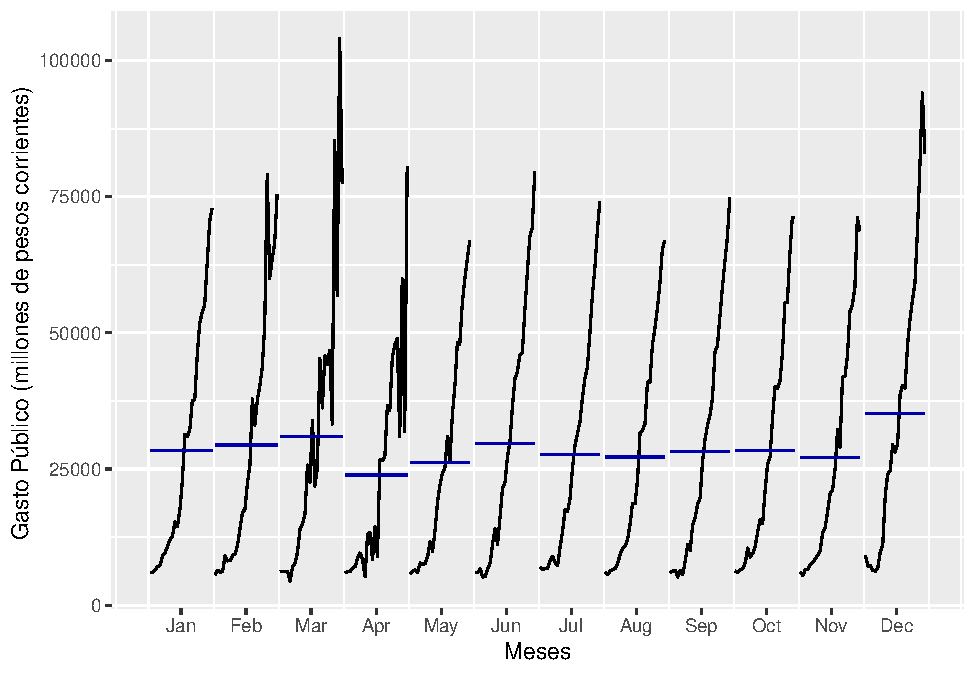
\includegraphics[width=0.75\linewidth]{informe_files/figure-latex/month_plot-1} 

}

\caption{\label{month_plot} Comportamiento mensual del Gasto Público entre 1999 y 2024.}\label{fig:month_plot}
\end{figure}

La figura \ref{seasonal_plot} muestra el comportamiento por año del
Gasto Público entre 1999 y 2024. En esta figura puede verse con mayor
claridad como se repiten los patrones año a año, lo cual, confirma la
estacionalidad resaltada en la figura anterior.

\begin{figure}[H]

{\centering 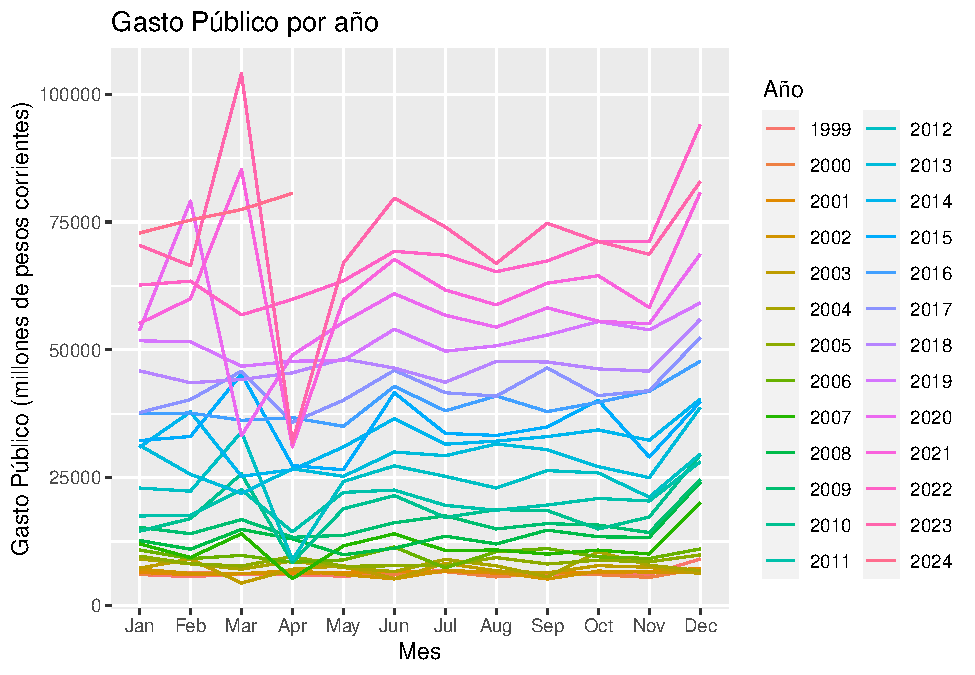
\includegraphics[width=0.75\linewidth]{informe_files/figure-latex/season_plot-1} 

}

\caption{\label{seasonal_plot} Comportamiento por año del Gasto Público entre 1999 y 2024.}\label{fig:season_plot}
\end{figure}

\hypertarget{metodologia}{%
\section{Metodología}\label{metodologia}}

El desarrollo de este trabajo esta basado en la metodología de Box y
Jenkins, en la construcción de modelos ARIMA para el análisis de series
de tiempo. Podemos dividir esta metodología en cuatro grandes etapas,
identificación, estimación, diagnostico y predicción. En la
identificación del modelo, consideraremos posibles transformaciones en
los datos, evaluaremos la aplicación de ciertos filtros con el objetivo
de obtener una serie estacional, con el uso de funciones de
autocorrelación y autocorrelación parcial, criterios de información,
diferentes test de raíces unitarias podremos obtener diferentes modelos
candidatos. Tras la estimación, un diagnostico con determinadas etapas
es realizado; y por último, aplicaremos predicciones sobre los mismos y
se evaluará su desempeño.

\hypertarget{identificaciuxf3n-del-modelo}{%
\subsection{Identificación del
modelo}\label{identificaciuxf3n-del-modelo}}

La transformación logarítimca de la serie, permite una homogenización de
la varianza y una mejor visualización de la tendencia. La figura
\ref{log_plot} muestra la evolución del logaritmo del Gasto Público
entre 1999 y 2024, que a diferencia de la serie original (figura
\ref{gasto_publico}), presenta una tendencia más estable y menos
volátil.

\begin{figure}[H]

{\centering 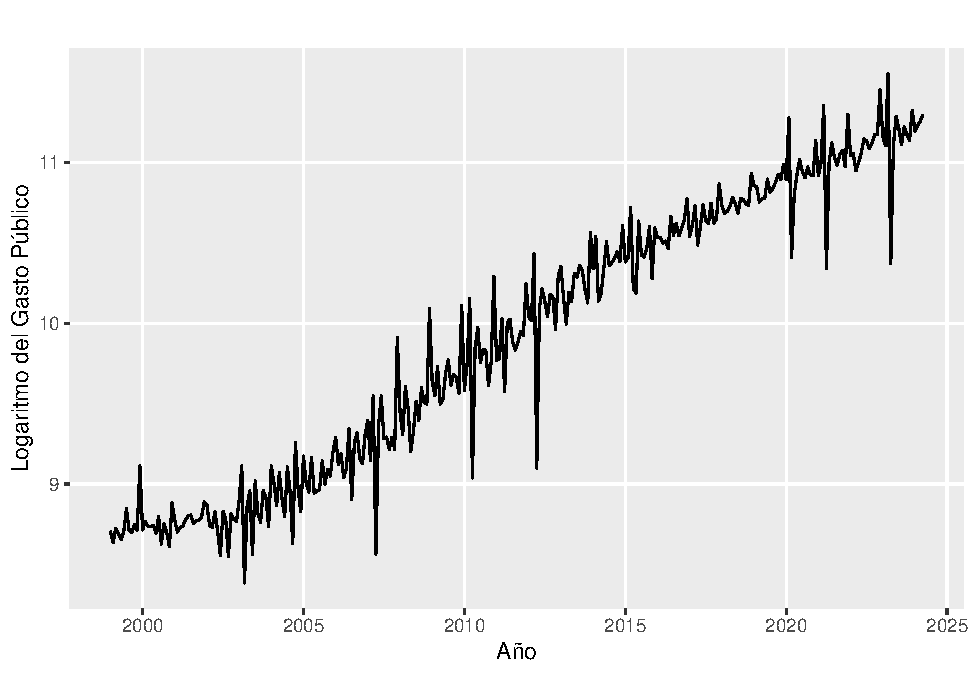
\includegraphics[width=0.75\linewidth]{informe_files/figure-latex/log_plot-1} 

}

\caption{\label{log_plot} Evolución del logaritmo del Gasto Público mensual entre 1999 y 2024.}\label{fig:log_plot}
\end{figure}

Obsérvese el autocorrelograma y el autocorrelograma parcial de la serie
en la figura \ref{fac_facp}. En la función de autocorrelación (FAC), se
observa una correlación significativa en los primeros rezagos, lo cual
sugiere la presencia de una tendencia en la serie, concluyendo que se
esta frente a una serie no estacionaria.

\begin{figure}[H]

{\centering 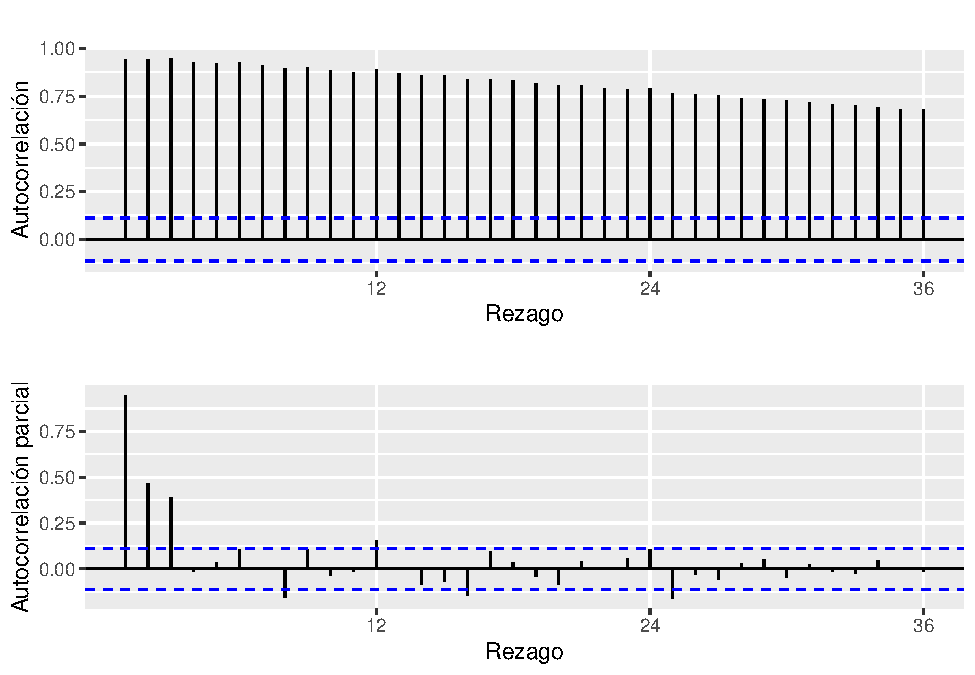
\includegraphics[width=0.75\linewidth]{informe_files/figure-latex/unnamed-chunk-1-1} 

}

\caption{\label{fac_facp} Funciones de Autocorrelación y Autocorrelación Parcial estimadas del logaritmo del Gasto Público.}\label{fig:unnamed-chunk-1}
\end{figure}

\hypertarget{pasos-a-seguir}{%
\subsubsection{Pasos a seguir}\label{pasos-a-seguir}}

Para modelar la tendencia podemos utilizar dos caminos alternativos:

\begin{itemize}
\item
  \textbf{Considerar una tendencia determinística TS}, esto implica
  considerar una tasa de crecimiento, \(\delta\), constante en el
  tiempo, remplazando la media del proceso estacionario como una función
  lineal del tiempo.
\item
  \textbf{Considerar un proceso de raíz unitaria DS}, esto implica
  determinar si existe una raíz unitaria en el polinomio autoregresivo,
  en caso que así sea, se debe de aplicar diferencias regulares en su
  medida justa para obtener un proceso estacionario.
\end{itemize}

Utilizar la primera opción no sería una buena alternativa ya que su
media no tiende a crecer a una tasa constante en el tiempo, veáse la
constante presente en la figura \ref{gasto_publico} y en la figura
\ref{log_plot} (tal vez no tanto en esta última).

\hypertarget{test-de-rauxedces-unitarias}{%
\subsubsection{Test de raíces
unitarias}\label{test-de-rauxedces-unitarias}}

Esta familia de test tiene como principal objetivo, detectar la
presencia de posibles raíces contenidas dentro del círculo unitario. Es
importante la detección de este tipo de raíces ya que esto impacta al
realizar nuestras inferencias e incumple el supuesto de estacionariedad,
además que en este caso la serie tendrá una variación que acompaña el
cambio en el tiempo, los shocks pasados tendrán efectos permanentes y el
comportamiento diverge hacia el infinito.

\hypertarget{test-de-dickey-fuller}{%
\paragraph{Test de Dickey-Fuller}\label{test-de-dickey-fuller}}

tiene como hipótesis nula que el proceso contiene una raíz unitaria y
por lo tanto que el proceso es no estacionario, mientras que la
alternativa es que no presenta raíz unitaria y por lo tanto, se cumple
el supuesto de estacionariedad. Para aplicar este test, se supone un
modelo autoregresivo de orden uno, se crean regresiones auxiliares donde
se puden incluir modelos con tendencia determinística o no, de la misma
manera que se hace con la incorporación de una constante.

Una consideración importante sobre este test es que se basa en que los
ruidos blancos de las regresiones auxiliares no se encuentra
correlacionados, en el caso que así sea existen alternativas propuestas
por Dickey-Fuller (1979) con un enfoque paramétrico que incluye los
rezagos de la variable dependiente.

La ecuación siguiente representa la solución paramétrica de DF (1979),
la regresión auxiliar con tendencia determínistica es la siguiente:

\[ \Delta Y_t = a_0 + a_2 t + \gamma Y_{t-1} + \sum_{j=1}^{k} \beta_j \Delta Y_{t-j} + \epsilon_t \]
donde \(Y_t\) es la serie de tiempo, \(t\) es el tiempo, \(\Delta\) es
el operador de diferencia, \(a_0\) y \(a_2\) son los coeficientes de la
regresión, \(\gamma\) es el coeficiente de la raíz unitaria, \(\beta_j\)
son los coeficientes de los rezagos y \(\epsilon_t\) es el término de
error.

Los contrastes de hipótesis que se realizan son los siguientes:

\begin{itemize}
\tightlist
\item
  Estadístico de prueba, \(\tau_3\) contrasta la hipótesis nula de que
  hay raíz unitaria, contra la alternativa de que no hay raíz unitaria,
  es decir es un proceso estacionario.
\end{itemize}

\begin{align*}
& \mathbf{H_0} : \gamma = 0 \\
& \mathbf{H_1} : \gamma < 1
\end{align*}

\begin{itemize}
\tightlist
\item
  Estadístico de prueba, \(\phi_2\) contrasta la hipótesis nula de que
  no tiene raíz unitaria, constante ni tendencia, contra la alternativa
  de que una de ellas es distinta de 0.
\end{itemize}

\begin{align*}
& \mathbf{H_0} : \gamma = a_0 = a_2 = 0 \\
& \mathbf{H_1} : \text{Al menos uno de ellos es distinto de 0.}
\end{align*}

\begin{itemize}
\tightlist
\item
  Estadístico de prueba, \(\phi_3\) contrasta la hipótesis nula de que
  no tiene raíz unitaria ni tendencia, contra la alternativa de que una
  de ellas es distinta de 0.
\end{itemize}

\begin{align*}
& \mathbf{H_0} : \gamma = a_2 = 0 \\
& \mathbf{H_1} : \text{Al menos uno de ellos es distinto de 0.}
\end{align*}

El estadístico \(\tau_3\) bajo la hipótesis nula sigue una distribución
t-Student, mientras que los estadísticos \(\phi_2\) y \(\phi_3\) de
prueba conjunta siguen una distribución F de Fisher.

Se aplica el test de Dickey-Fuller sobre el logarítmo del gasto público.
El test con tendencia y 12 rézagos significativos obtuvo los siguientes
resultados para un nivel de significación al 5\%. El estadístico \(
\tau_3 = -2.33\) y un \(p-valor=-3.42\), no se rechaza \(H_0\) y
por lo tanto la serie tiene una raíz unitaria. Luego, \(\phi_2 = 20.29\)
y un \(p-valor=4.71\), se rechaza \(H_0\), por lo tanto al menos uno de
\(\gamma = a_0 = a_2\) es distinto de 0, es decir o presenta
constante, o presenta tendencia, porque ya se constrasto que
\(\gamma = 0\). Por último, \(\phi_3 = 3.13\) y un \(p-valor=6.30\), no
se rechaza \(H_0\), en conclusión la serie no tiene raíz unitaria ni
tendencia.

Por lo tanto, dado los 3 contrastes se concluye que la serie tiene raíz
unitaria, no tiene tendencia y presenta constante. Esto sugiere que la
serie no es estacionaria y se debe de aplicar una diferencia regular
para obtener un proceso estacionario.

Se aplica una diferencia regular a la serie dada la sugerencia del test,
la figura \ref{diff_plot} muestra la evolución de la primera diferencia
regular del logaritmo del Gasto Público entre 1999 y 2024. La serie
diferenciada presenta una tendencia más estable y menos volátil que la
serie original, lo cual sugiere que la diferenciación ha logrado
estacionarizar la serie.

\[(1-L)Ln(gasto)\]

\begin{figure}[H]

{\centering 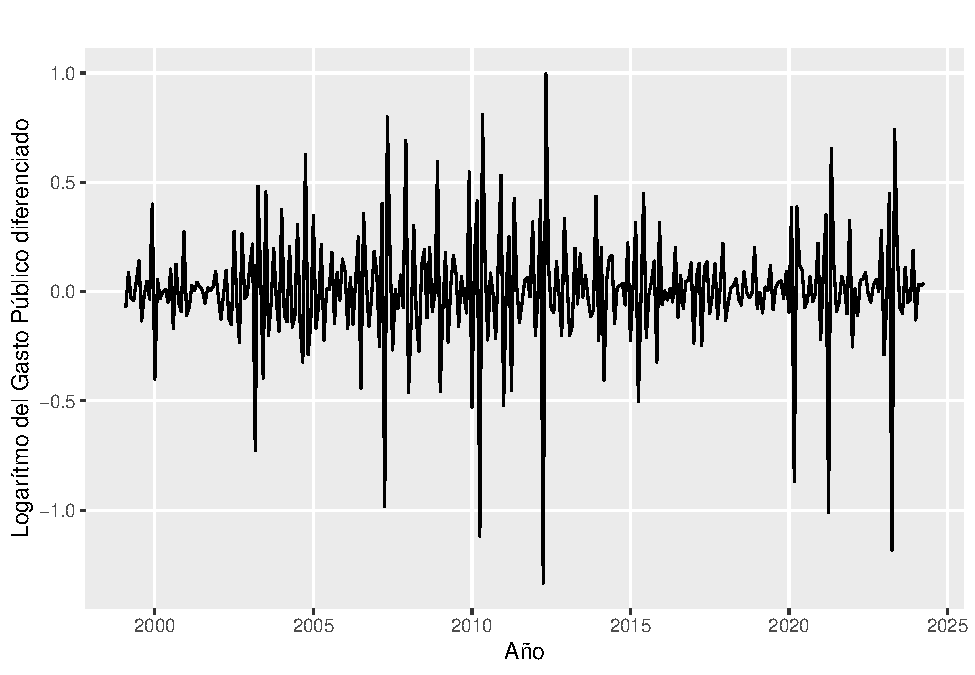
\includegraphics[width=0.75\linewidth]{informe_files/figure-latex/unnamed-chunk-3-1} 

}

\caption{\label{diff_plot} Evolución de la primera diferencia regular del logaritmo del Gasto Público mensual entre 1999 y 2024.}\label{fig:unnamed-chunk-3}
\end{figure}

Los nuevos autocorrelogramas pueden verse en la figura
\ref{fac_facp_diff}. En ambas funciones se observa una convergencia, lo
cual sugiere que la serie diferenciada es estacionaria.

\begin{figure}[H]

{\centering 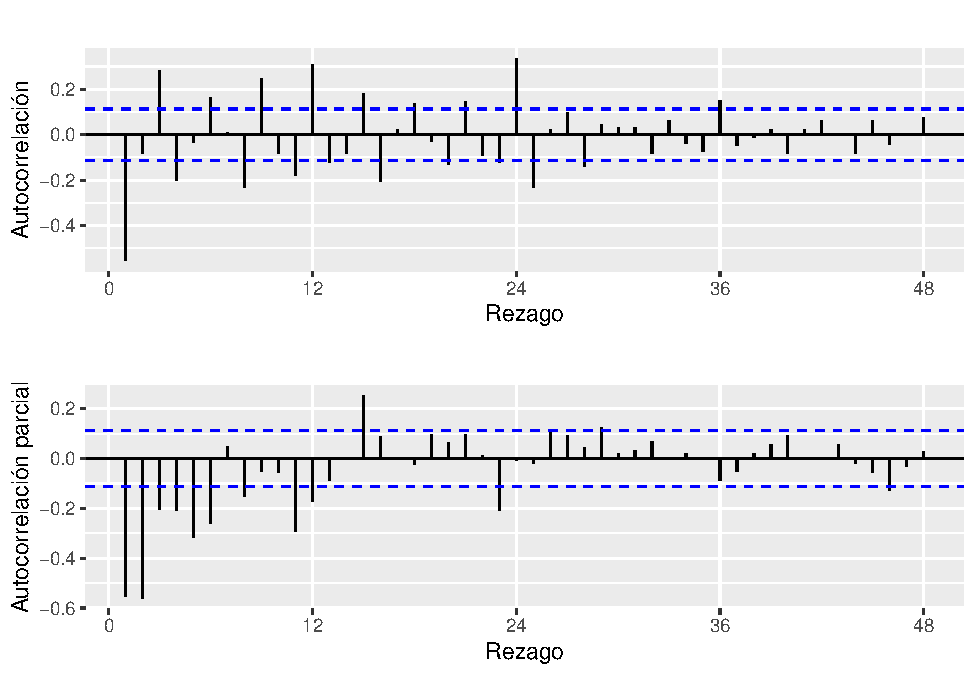
\includegraphics[width=0.75\linewidth]{informe_files/figure-latex/unnamed-chunk-4-1} 

}

\caption{\label{fac_facp_diff} Funciones de Autocorrelación y Autocorrelación Parcial estimadas para la primera diferencia regular del logaritmo del Gasto Público.}\label{fig:unnamed-chunk-4}
\end{figure}

Sin embargo, la serie diferenciada presenta una estacionalidad marcada,
como se observa en la figura \ref{seasonal_plot}, existe una
estacionalidad que se repite año a año. En los rezagos 12, 24, 36 de la
FAC se ve una significancia, lo cual sugiere que la estacionalidad no ha
sido eliminada con la diferenciación regular. Una diferencia estacional
anual es aplicada para estacionarizar la serie.

\[(1-L^{12}) Ln(gasto)\] La figura \ref{dif-est-gasto}, cotenida en el
apéndice, contiene la serie con la diferencia estacional. La
diferenciación por si sola logra estacionarizar la serie, veáse la FAC y
FACP en la figura \ref{fac_facp_estac}.

\begin{figure}[H]

{\centering 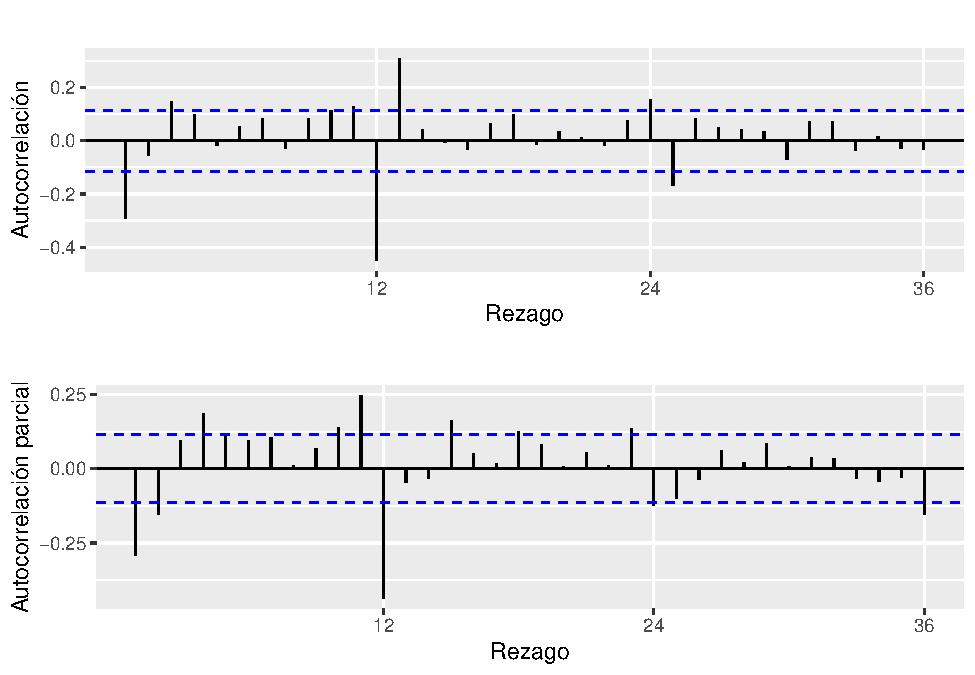
\includegraphics[width=0.75\linewidth]{informe_files/figure-latex/unnamed-chunk-5-1} 

}

\caption{\label{fac_facp_estac} Funciones de Autocorrelación y Autocorrelación Parcial estimadas para la primera diferencia estacional del logaritmo del Gasto Público (1999-2024).}\label{fig:unnamed-chunk-5}
\end{figure}

La diferencia estacional, elimina la estacionalidad presente y logrando
convergencia en ambas funciones de autocorrelación, permitiendo
estacionarizar la serie. A partir de estos autocorrelogramas, se procede
a la identificación de un modelo SARIMA, identificando dos modelos
posibles, SARIMA(0,0,1)(0,1,1) y SARIMA(0,0,1)(1,1,0).

Estos modelos surgen de los rezagos significativos presentes en las
funciones. Con respecto a la parte regular de modelo, se puede observar
una rápida convergencia de la serie en la FAC, mientras que en la FACP
dicha convergencia no es tan rápida, lo cual sugiere un modelo que
contiene solo parte MA; el rezago 1 significativo de la FAC sugiere
\(q=1\) y \(p=d=0\) en un modelo SARIMA(p,d,q)(P,D,Q). Con respecto a la
parte estacional, los rezagos múltiplos de 12 son los relevantes en la
FAC y FACP, ambas funciones presentan el primer rezago (rezago 12)
significativo, y una convergencia medianamente rápida. Esto sugiere
probar dos posibilidades \(P=1\) o \(Q=1\) siendo \(D=1\).

Finalmente, se prueban ambas diferencias en la serie, regular y
estacional, veáse la figura \ref{difdif-est-gasto} en el apéndice y en
la figura \ref{dd_fac_facp}:

\[(1-L)(1-L^{12}) Ln(gasto)\]

\begin{figure}[H]

{\centering 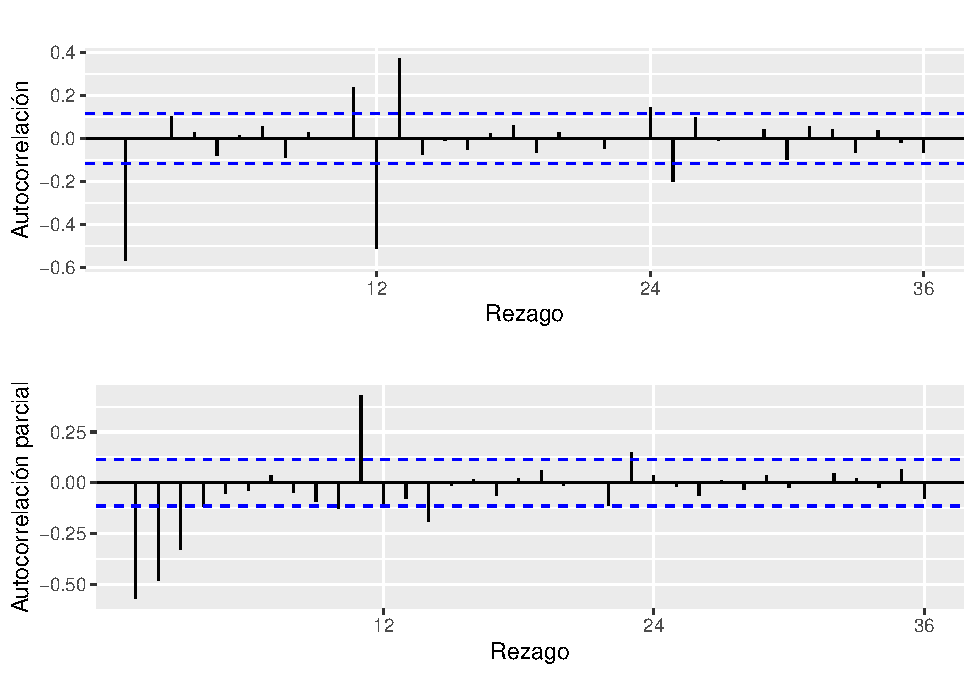
\includegraphics[width=0.75\linewidth]{informe_files/figure-latex/unnamed-chunk-6-1} 

}

\caption{\label{dd_fac_facp} Funciones de Autocorrelación y Autocorrelación Parcial estimadas para la primera diferencia regular de la primera diferencia estacional del logaritmo del Gasto Público.}\label{fig:unnamed-chunk-6}
\end{figure}

La convergencia de las funciones es mas consistente que en la serie con
diferencia estacional únicamente. A partir de estas funciones se
identifican 2 modelos adicionales, SARIMA(0,1,2)(1,1,0) y
SARIMA(0,1,1)(0,1,1).

En este caso al haber ambas diferencias los parámetros \(d=1\) y \(D=1\)
son fijos. Con respecto a la parte regular, la FACP presenta los
primeros tres rezagos significativos, sin embargo se descarta un modelo
con parte AR de orden tan grande dado que la FAC no presenta un ruido
tan grande; de haber parte AR, la FAC no presentaria una convergencia
tan rápida como tiene a partir del rezago 2. En cambio, la convergencia
de la FACP es más lenta, lo cual sugiere un modelo con parte MA de orden
1 e incluso 2, por lo tanto \(q={1,2}\). Con respecto a la parte
estacional, las conclusiones son las mismas a la de la figura
\ref{fac_facp_estac}, la FAC y la FACP presenta el primer rezago
significativo dando lugar a dos posibilidades \(P=1\) o \(Q=1\).

\hypertarget{estimaciuxf3n-del-modelo}{%
\subsection{Estimación del modelo}\label{estimaciuxf3n-del-modelo}}

La etapa de identificación ha identificado 4 modelos posibles para
modelar la serie de Gasto Público. Estos modelos son en esta parte
estimados y comparados. Adicionalmente es incorporada al modelo una
variable regresora, los días de turismo, con el objetivo de capturar la
variabilidad de la serie generada en los marzos y abril de cada año, que
coincidie con el pago de los aguinaldos de los empleados públicos. La
figura \ref{gasto_2009-2013} representa la evolución del logaritmo del
Gasto Público entre enero 2009 y diciembre 2012, con las líneas
verticales punteadas marcando los meses de marzo y abril de cada año.

\begin{figure}[H]

{\centering 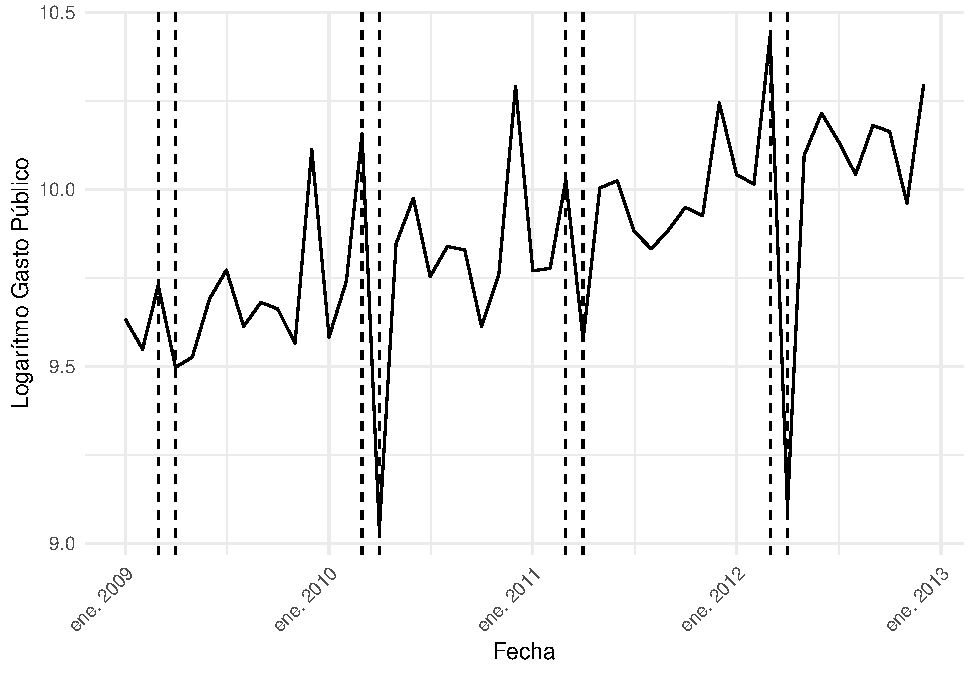
\includegraphics[width=0.85\linewidth]{informe_files/figure-latex/gasto_2009-2012-1} 

}

\caption{\label{gasto_2009-2013} Evolución del Logarítmo del Gasto Público mensual entre enero 2009 y diciembre 2012.}\label{fig:gasto_2009-2012}
\end{figure}

Dependiendo de cuando caen los días de turismo, determina el mes en el
que se efectuará el pago de los aguinaldos de los empleados públicos.
Esto puede generar un pago anticipado de los aguinaldos en determinado
mes, generando un alto gasto, y un gasto mucho menor al mes siguiente.
El cuadro \ref{tab:turismo} muestra los dias de turismo de cada año
entre 2009-2012:

\begin{table}[H]
\centering
\begin{tabular}{c c c c c}
\hline
 & 2009 & 2010 & 2011 & 2012 \\ \hline
Marzo & 0 & 3 & 0 & 0 \\ 
Abril & 7 & 4 & 7 & 7 \\ \hline
\end{tabular}
\caption{Días de tursimo en marzo y abril de 2009 a 2012.}
\label{tab:turismo}
\end{table}

Por lo tanto, se incorpora esta variable al modelo para capturar la
variabilidad de la serie en los meses de marzo y abril de cada año.

El cuadro \ref{tab:models}, es un resúmen de la estimación de los 4
modelos SARIMA identificados, proporciona la varianza del modelo y la
significancia de sus componentes.

\begin{table}[H]
\centering
\begin{tabular}{c c c c}
\hline
Modelo & SARIMA(p,d,q)(P,D,Q) + turismo & $\sigma^2$ & Significancia de los componentes \\ \hline
1 & (0,0,1)(0,1,1) & 0.0493 & MA 1 no significativo \\ 
2 & (0,0,1)(1,1,0) & 0.0484 & MA 1 no significativo \\ 
3 & (0,1,2)(1,1,0) & 0.0240 & Todos significativos \\ 
4 & (0,1,1)(0,1,1) & 0.0271 & Todos significativos \\ \hline
\end{tabular}
\caption{Estimación de modelos SARIMA.}
\label{tab:models}
\end{table}

Los dos modelos que incluyen únicamente la diferencia estacional,
aparentan ser peores que los modelos con diferencias regular y
estacional en términos de varianza del modelo, a su vez el componente MA
de orden 1 en la parte regular de los dos primeros modelos, suele ser
rechazada al 5\% de nivel de significación.

Este resultado se acompaña del Test de Dickey-Fuller, el cual sugiere
que la serie presenta una diferencia regular, y los modelos 1 y 2 no
contemplan.

\hypertarget{diagnuxf3stico}{%
\subsection{Diagnóstico}\label{diagnuxf3stico}}

En esta etapa, los 4 modelos estimados son diagnosticados para verificar
si cumplen con los supuestos de ruido blanco es decir incorrelación y
normalidad de los resiudos.

El análisis de las funciones de autocorrelación y autocorrelación
parcial de los residuos permite observar la autocorrelación de los
mismos, y acompañado del test de Ljung-Box, se verifica la
incorrelación.

Por otro lado los tests de Shapiro-Wilks y Jarque-Bera, permiten
verificar la normalidad de los residuos.

Las figuras \ref{residuos1}, \ref{residuos2}, \ref{residuos3},
\ref{residuos4} contenidas en el apéndice, muestran los residuos y los
residuos estandarizados de los modelos 1, 2, 3 y 4 respectivamente. En
todos los casos, los residuos estandarizados presentan observaciones que
superan las 3 desviaciones estándar, dando lugar a la presencia de
puntos atípicos en todos los modelos que se tienen que intervenir.

Adicionalmente, las figuras \ref{facyp_r1}, \ref{facyp_r2},
\ref{facyp_r3}, \ref{facyp_r4} contenidas en el apéndice, muestran las
funciones de autocorrelación y autocorrelación parcial de los residuos
de los modelos 1, 2, 3 y 4 respectivamente. En todos los casos, pueden
observarse rézagos significativos lo cual anticipa la ausencia de
incorrelación en los residuos. El test de Ljung-Box contrastará esta
hipótesis.

Veánse los resultados de la incorrelación y normalidad de los resiudos
en el cuadro \ref{tab:diagnostico}.

\begin{table}[H]
\centering
\begin{tabular}{c c c c}
\hline
Modelo & SARIMA(p,d,q)(P,D,Q) + turismo & Incorrelación & Normalidad \\ \hline
1 & (0,0,1)(0,1,1) & No & No \\ 
2 & (0,0,1)(1,1,0) & No & No \\ 
3 & (0,1,2)(1,1,0) & No & No \\ 
4 & (0,1,1)(0,1,1) & No & No \\ \hline
\end{tabular}
\caption{Diagnostico de modelos SARIMA.}
\label{tab:diagnostico}
\end{table}

En base al cuadro anterior, podemos ver que todos los modelos rechazan
la hipótesis nula, \(H_0\) de Ljung-Box para los primeros 24 rezagos,
indiciando problemas de ajuste.

De forma similar, todos los modelos presentados tienen problema con la
normalidad de los residuos, ya que en absolutamente todos los modelos
existe evidencia suficiente para decidir que los residuos no provienen
de una distribución normal.

A partir de esto, se procede a detectar e intervenir datos atípticos
presentes en la serie, una vez hecho se reestiman los modelos con la
inclusión de los outliers detectados. Para la detección de outliers, se
utiliza la función \texttt{tso} del paquete \texttt{tsoutliers}.

Los outliers detectados para cada modelo son las siguientes
observaciones:

\begin{itemize}
\tightlist
\item
  Modelo 1

  \begin{itemize}
  \tightlist
  \item
    AO: 51, 100, 136, 160, 195, 255, 267, 280, 304.
  \item
    LS: 117, 159.
  \item
    TC: 254
  \end{itemize}
\item
  Modelo 2

  \begin{itemize}
  \tightlist
  \item
    AO: 51, 100, 136, 160, 195, 255, 267, 280, 304.
  \item
    TC: 159, 254, 291.
  \end{itemize}
\item
  Modelo 3

  \begin{itemize}
  \tightlist
  \item
    AO: 100, 160, 292.
  \end{itemize}
\item
  Modelo 4

  \begin{itemize}
  \tightlist
  \item
    AO: 51, 100, 136, 160, 195, 255, 268, 279, 292.
  \end{itemize}
\end{itemize}

Los outliers detectados en cada modelo son en gran parte de tipo aditivo
(AO), algunos de ellos se repiten en todos los modelos. El modelo 1
identifica dos casos donde sugiere cambios de nivel (LS), que se
corresponden a las fechas 09/2008 y 03/2012, una de estas fechas puede
observarse en la figura \ref{gasto_2009-2013}, esta sugerencia en la
serie no aparenta ser realmente un cambio de nivel sino tan solo un
atípico aditivo. Los modelos 1 y 2 presentan observaciones donde se
sugiere atípicos de cambios transitorios (TC). El modelo 3 es el que
requiere menor intervenciones con solo 3 outliers detectados
correspondientes a las meses de abril de los años 2007, 2012 y 2023,
mientras que el modelo 1 es el que requiere mayor intervenciones. Un
modelo que requiere menos intervenciones es preferible ante otro con una
mayor cantidad de intervenciones.

Los modelos identificados, son reestimados con la inclusión de los
outliers detectados. Los resultados de la reestimación se presentan en
el cuadro \ref{tab:models2}.

\begin{table}[H]
\centering
\resizebox{1\textwidth}{!}{
\begin{tabular}{c c c c}
\hline
Modelo & SARIMA(p,d,q)(P,D,Q) + turismo + outliers & $\sigma^2$ & Significancia de los componentes \\ \hline
1 & (0,0,1)(0,1,1) & 0.0227 & s\_MA 1 no significativo \\ 
2 & (0,0,1)(1,1,0) & 0.0226 & Todos significativos \\ 
3 & (0,1,2)(1,1,0) & 0.0205 & Regresor turismo no significativo \\ 
4 & (0,1,1)(0,1,1) & 0.0156 & Todos significativos \\ \hline
\end{tabular}
}
\caption{Reestimación de modelos SARIMA con intervención de outliers.}
\label{tab:models2}
\end{table}

En base al cuadro anterior, podemos ver que todos los modelos
reestimados presentan una varianza del modelo menor que los modelos
originales, lo cual es un indicador de un mejor ajuste. En cuanto a la
significancia de los componentes, el modelo 1 presenta un componente MA
de orden 1 de la parte estacional no significativo, mientras que el
modelo 3 presenta el regresor turismo no significativo.

Se vuelven a reestimar los modelos 1 y 3 con los ajustes mencionados en
el parrafo anterior. Una vez modificados se obtienen los resultados
presentados en el cuadro \ref{tab:models3}.

\begin{table}[H]
\centering
\resizebox{1\textwidth}{!}{
\begin{tabular}{c c c c}
\hline
Modelo & SARIMA(p,d,q)(P,D,Q) + outliers & $\sigma^2$ & Significancia de los componentes \\ \hline
1 & (0,0,1)(0,1,0) + turismo & 0.0226 & Todos significativos \\ 
3 & (0,1,2)(1,1,0) & 0.0205 & Todos significativos \\ \hline
\end{tabular}
}
\caption{Reestimación de modelos SARIMA con intervención de outliers.}
\label{tab:models3}
\end{table}

Se vuelve a estudiar la autocorrelación y normalidad de los residuos de
los modelos reestimados. Los resultados se presentan en el cuadro
\ref{tab:diagnostico2}.

\begin{table}[H]
\centering
\begin{tabular}{c c c c}
\hline
Modelo & SARIMA(p,d,q)(P,D,Q) + outliers & Incorrelación & Normalidad \\ \hline
1 & (0,0,1)(0,1,0) + tursimo & No & No \\ 
2 & (0,0,1)(1,1,0) + turismo & No & No \\ 
3 & (0,1,2)(1,1,0) & No & No \\ 
4 & (0,1,1)(0,1,1) + turismo & No & No \\ \hline
\end{tabular}
\caption{Diagnosticos de modelos SARIMA.}
\label{tab:diagnostico2}
\end{table}

De forma similar al primer diagnostico, los modelos reestimados
presentan problemas de incorrelación y normalidad en los residuos.

En el apéndice, se encuentra la figura \ref{norms} que presenta los
histogramas de los residuos junto a las densidades de una distribución
normal basada en los resiudos de cada modelos; en todos los modelos los
residuos se asemejan a una distribución normal, sin embargo el test de
Shapiro-Wilks rechaza la hipótesis de normalidad.

\hypertarget{predicciuxf3n}{%
\subsection{Predicción}\label{predicciuxf3n}}

En esta etapa, se procede a realizar la predicción de la serie Gasto
Público. Al momento de realizar una predicción hay cierto puntos que
deben tenerse en cuenta antes de comenzar. Primero la función de pérdida
asociada, debe ser adecuada al problema que se plantea en particualr. La
función de pérdida que se utiliza en esta ocasión es la simétrica, es
decir que la penalización de un error de predicción es igual para un
error positivo que para un error negativo.

Para graficar la predicción, es utilizado el gráfico de \emph{Fan
Chart}, este gráfico permite visualizar la incertidumbre de las
predicciones, y reflejar la variabilidad de las predicciones.

El horizonte de predicción seleccionado es a 1 año porque se determinó
que la serie tiene cierta estacionalidad anual, dado esto, se considera
que el horizonte a un año es un horizonte de predicción adecuado. Por
ende se selecciona como conjunto de entrenamiento a las observaciones
hasta abril 2023, dejando al conjunto de mayo 2023 hasta abril 2024 como
conjunto de validación.

Se utiliza la función \texttt{forecast} del paquete con su mismo nombre
para realizar las predicciones.

Para evaluar las predicciones se utiliza las métricas de error absoluto
medio (MAE), error absoluto medio porcentual (MAPE) y el error absoluto
medio escalado (MASE). Estas métricas permiten evaluar la calidad de las
predicciones realizadas en el conjunto de entrenamiento y testeo. El MAE
nos dice cuánto se desvía en promedio la predicción del valor real, el
MAPE nos dice cuánto se desvía en promedio la predicción del valor real
en términos porcentuales y el MASE nos dice la media del error absoluto
de las predicciones, escalada por el MAE del conjunto de entrenamiento;
para las tres métricas, un valor más cercano a cero indica una mejor
predicción.

Las figuras \ref{fig:unnamed-chunk-21} y \ref{fig:unnamed-chunk-22} representan los horizontes de prediccion de los modelos 1 y 2, y 3 y 4 respectivamente.

\begin{figure}[H]

{\centering 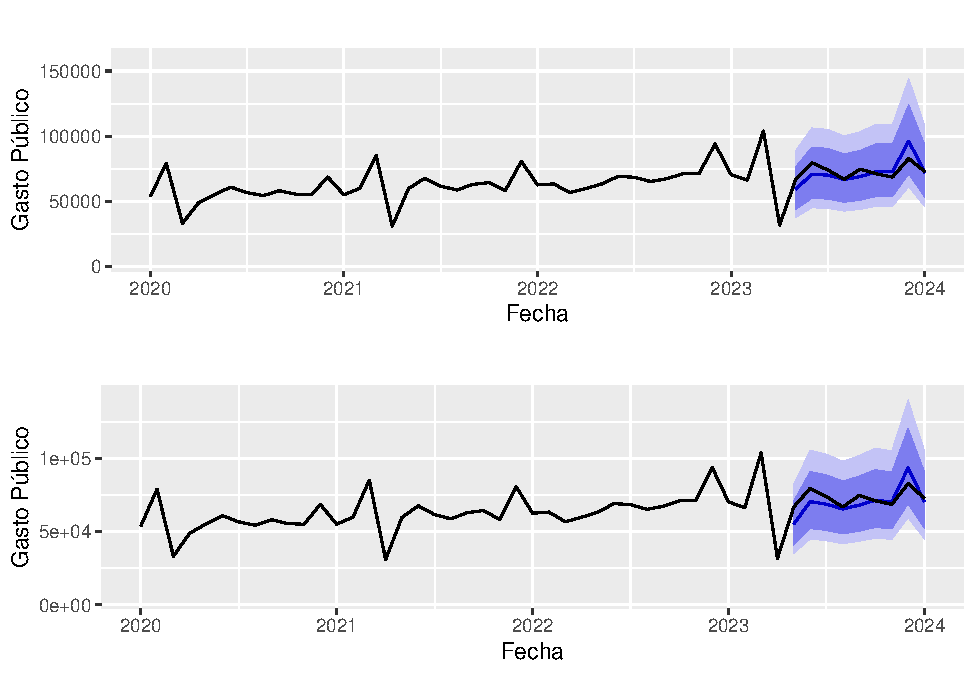
\includegraphics[width=0.95\linewidth]{informe_files/figure-latex/unnamed-chunk-21-1}

}

\caption{\label{fig:unnamed-chunk-21} Predicciones en el conjunto de prueba del Gasto
Público, para los modelos 1 y 2 respectivamente. La línea azul
corresponde a las predicciones y la negra a los datos reales. El azul
mas claro correspode al intervalo de predicción al 95\% de confianza y
la mas oscura al 80\%.}

\end{figure}


\begin{figure}[H]

{\centering 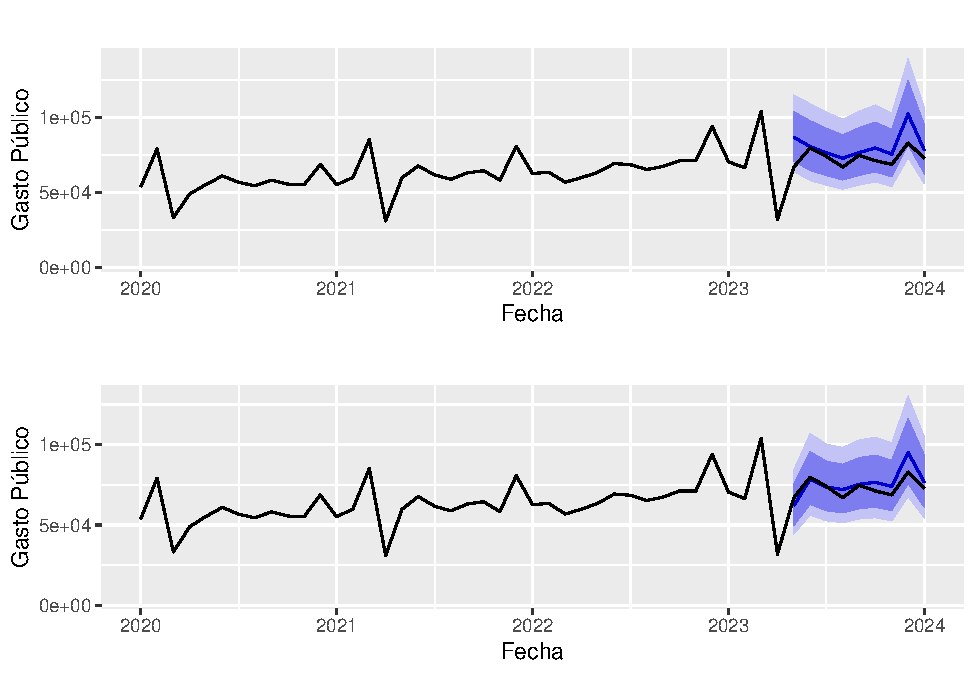
\includegraphics[width=0.95\linewidth]{informe_files/figure-latex/unnamed-chunk-22-1}

}

\caption{\label{fig:unnamed-chunk-22} Predicciones en el conjunto de prueba del Gasto
Público, para los modelos 3 y 4 respectivamente. La línea azul
corresponde a las predicciones y la negra a los datos reales. El azul
mas claro correspode al intervalo de predicción al 95\% de confianza y
la mas oscura al 80\%.}

\end{figure}

\begin{table}[H]
\centering
\begin{tabular}{c c c c c c}
\hline
Modelo & Conjunto & MAE & MAPE & MASE \\ \hline
1 & Training  & 3541 & 12.85 & 0.868 \\ 
1 & Test      & 10870 & 13.98 & 2.664 \\ \hline
2 & Training  & 3565 & 13.10 & 0.874 \\ 
2 & Test      & 9909 & 12.84 & 2.429 \\ \hline
3 & Training  & 2757 & 10.92 & 0.676 \\ 
3 & Test      & 9333 & 12.45 & 2.288 \\ \hline
4 & Training  & 2729 & 10.87 & 0.669 \\ 
4 & Test      & 6829 & 8.93 & 1.674 \\ \hline
\end{tabular}
\caption{Resultados de error de predicción para los diferentes modelos.}
\label{tab:metricas}
\end{table}

Las predicciones realizadas en el conjunto de testeo, presentan un error
absoluto medio (MAE) de 10870, 9909, 9333 y 6829 para los modelos 1, 2,
3 y 4 respectivamente. El error absoluto medio porcentual (MAPE) es de
13.98, 12.84, 12.45 y 9.42 para los modelos 1, 2, 3 y 4 respectivamente.
Y el error absoluto medio escalado (MASE) es de 2.664, 2.429, 2.288 y
1.674 para los modelos 1, 2, 3 y 4 respectivamente. En base a las
métricas de error, el modelo 4 es el que presenta un mejor desempeño en
el conjunto de testeo y en el conjunto de entrenamiento para las 3
métricas de error de predicción, seguido por el modelo 3, 2 y 1
respectivamente.

\hypertarget{comentarios}{%
\section{Comentarios Finales}\label{comentarios}}

En base a los resultados obtenidos, se puede concluir que el modelo 4
(entre los presentados) es el que presenta un mejor desempeño en los
datos. Este modelo es un SARIMA(0,1,1)(0,1,1) con un regresor turismo y
la inclusión de outliers detectados.

Se ha logrado llegar a resultados positivos, mas alla de la falta de
cumplimiento de los supuestos de los residuos respecto a la
incorrelación y normalidad de los residuos. Los puntos atípicos
presentes en la serie, han sido correctamente identificados y tratados
en los modelos, lo cual ha permitido mejorar la calidad de las
estimaciones.

Hubiese estado bueno que al identificar los outliers aparte de haber
mejorado la estimación, hubiese ayudado al cumplimiento de la
incorrelación y normalidad de los residuos.

La predicción realizada en el conjunto de testeo, respondió
correctamente, presentando un error de predicción dentro de las
expectativas. El modelo 3 presenta una predicción rara de la primer
observación que solo queda contenida en el intervalo de predicción al
95\% de confianza, se desconoce el motivo de este comportamiento.

A efectos futuros, se sugiere probar las siguientes combinaciones de
modelos que quedaron pendientes de estimar y diagnosticar,
SARIMA(p,d,q)(P,D,Q): 
  \begin{itemize}
  \tightlist
  \item
    (0,1,2) (0,1,1)
  \item
    (0,1,1) (1,1,0)
  \end{itemize}

\newpage

\hypertarget{referencias}{%
\section*{Referencias}\label{referencias}}
\addcontentsline{toc}{section}{Referencias}

\hypertarget{refs}{}
\begin{CSLReferences}{1}{0}
\leavevmode\vadjust pre{\hypertarget{ref-box1994time}{}}%
Box, G. E. P., G. M. Jenkins, y G. C. Reinsel. 1994. \emph{Time Series
Analysis; Forecasting and Control}. 3rd ed. Englewood Cliff, New Jersey:
Prentice Hall.

\leavevmode\vadjust pre{\hypertarget{ref-MEFUruguay}{}}%
Ministerio de Economía y Finanzas. 2024. {«{Información y Resultados del
Sector Público}»}.
\url{https://www.gub.uy/ministerio-economia-finanzas/datos-y-estadisticas/estadisticas/informacion-resultados-del-sector-publico}.

\end{CSLReferences}

\hypertarget{apuxe9ndice}{%
\section*{Apéndice}\label{apuxe9ndice}}
\addcontentsline{toc}{section}{Apéndice}

El informe viene acompañado de 1 carpeta en formato .zip,
que contiene todo lo necesario para replicar el trabajo. 

\begin{figure}[H]

{\centering 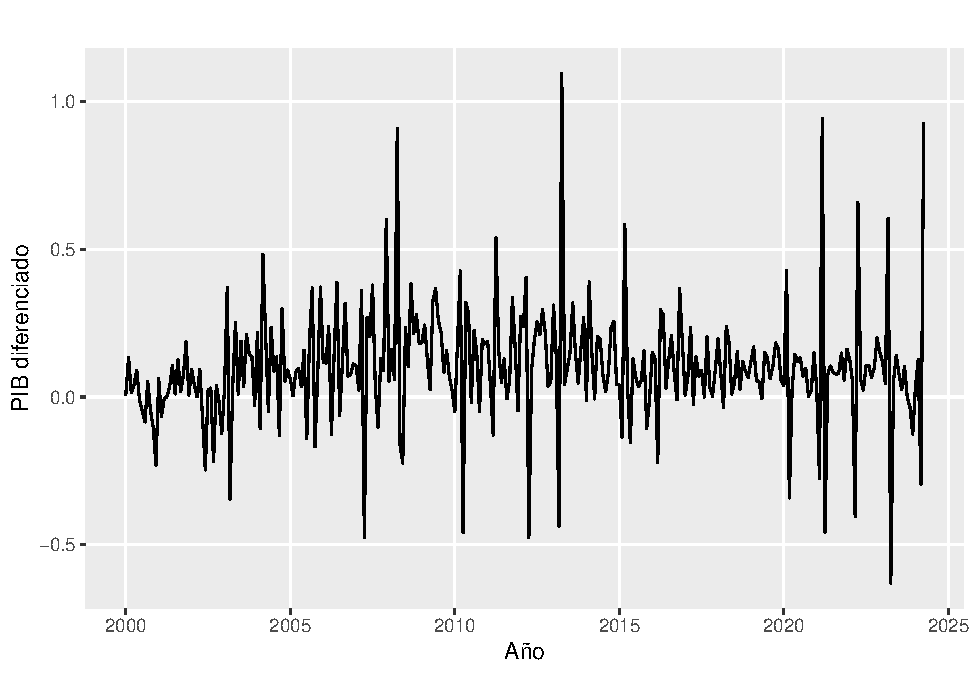
\includegraphics[width=0.75\linewidth]{informe_files/figure-latex/unnamed-chunk-24-1} 

}

\caption{\label{dif-est-gasto} Evolución de la primera diferencia estacional del logaritmo del Gasto Público.}\label{fig:unnamed-chunk-24}
\end{figure}

\begin{figure}[H]

{\centering 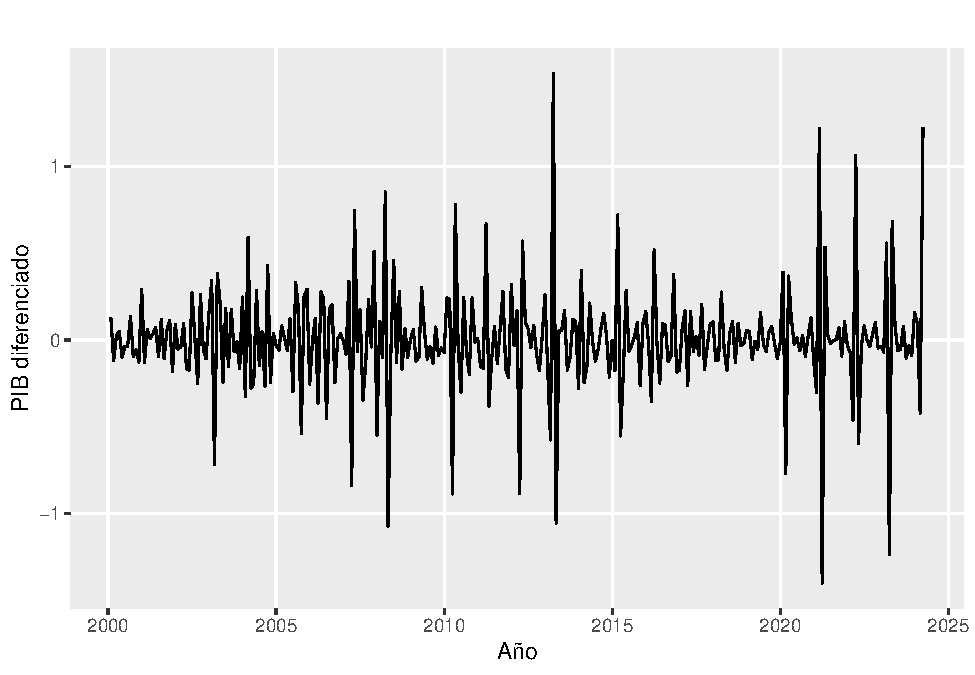
\includegraphics[width=0.75\linewidth]{informe_files/figure-latex/unnamed-chunk-25-1} 

}

\caption{\label{difdif-est-gasto} Evolución de la primera diferencia regular de la primera diferencia estacional del logaritmo del Gasto Público.}\label{fig:unnamed-chunk-25}
\end{figure}

\begin{figure}[H]

{\centering 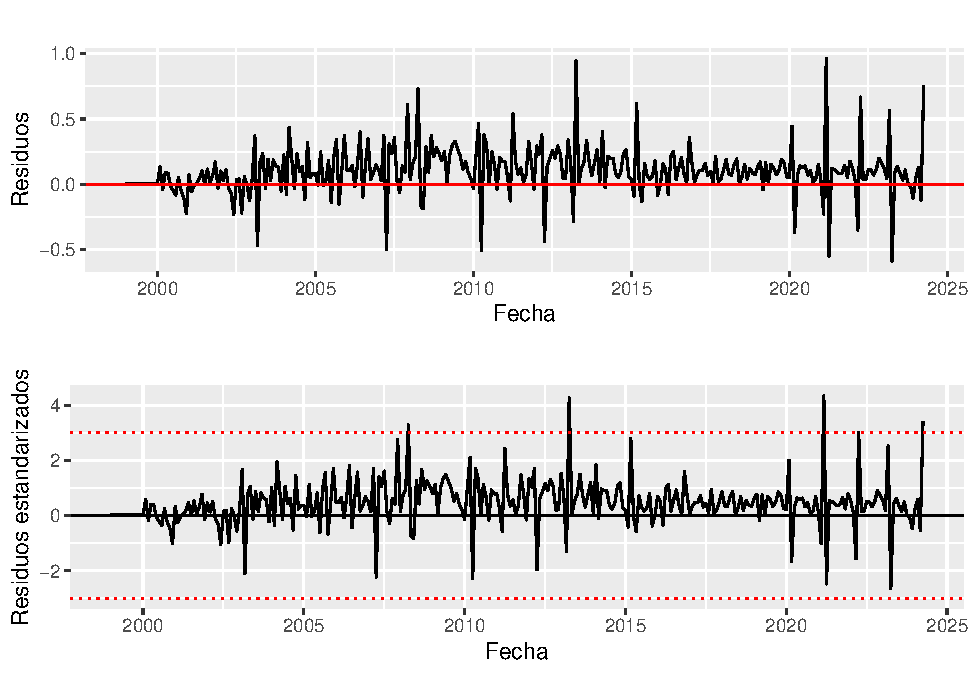
\includegraphics[width=0.75\linewidth]{informe_files/figure-latex/unnamed-chunk-26-1} 

}

\caption{\label{residuos1} Residuos normales y estandarizados de un modelo SARIMA(0,0,1)(0,1,1) para el logaritmo del Gasto Público.}\label{fig:unnamed-chunk-26}
\end{figure}

\begin{figure}[H]

{\centering 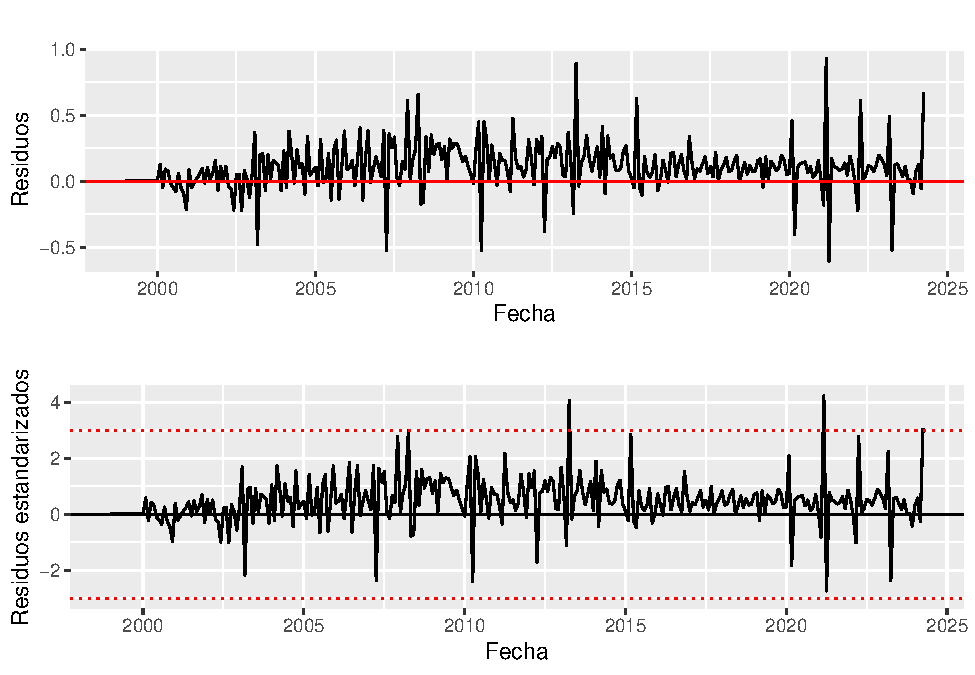
\includegraphics[width=0.75\linewidth]{informe_files/figure-latex/unnamed-chunk-27-1} 

}

\caption{\label{residuos2} Residuos normales y estandarizados de un modelo SARIMA(0,0,1)(1,1,0) para el logaritmo del Gasto Público.}\label{fig:unnamed-chunk-27}
\end{figure}

\begin{figure}[H]

{\centering 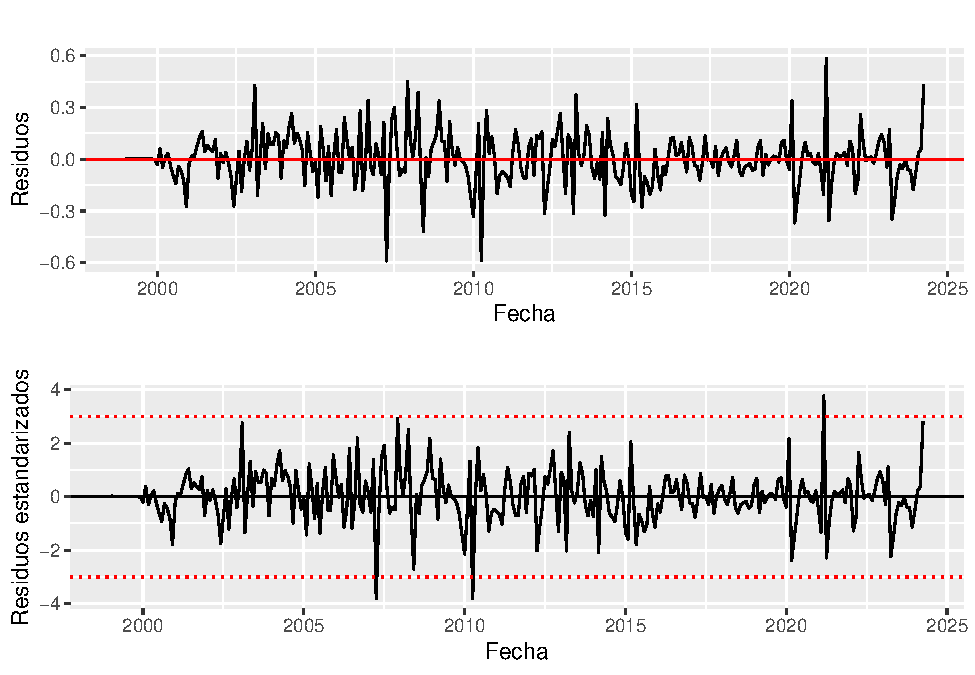
\includegraphics[width=0.75\linewidth]{informe_files/figure-latex/unnamed-chunk-28-1} 

}

\caption{\label{residuos3} Residuos normales y estandarizados de un modelo SARIMA(0,1,2)(1,1,0) para el logaritmo del Gasto Público.}\label{fig:unnamed-chunk-28}
\end{figure}

\begin{figure}[H]

{\centering 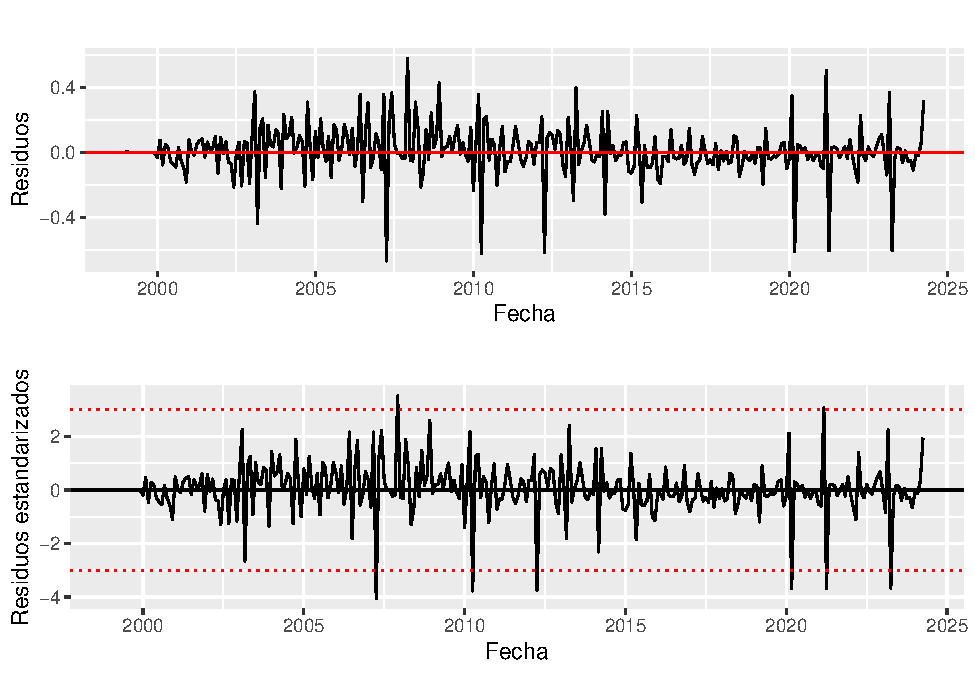
\includegraphics[width=0.75\linewidth]{informe_files/figure-latex/unnamed-chunk-29-1} 

}

\caption{\label{residuos4} Residuos normales y estandarizados de un modelo SARIMA(0,1,1)(0,1,1) para el logaritmo del Gasto Público.}\label{fig:unnamed-chunk-29}
\end{figure}

\begin{figure}[H]

{\centering 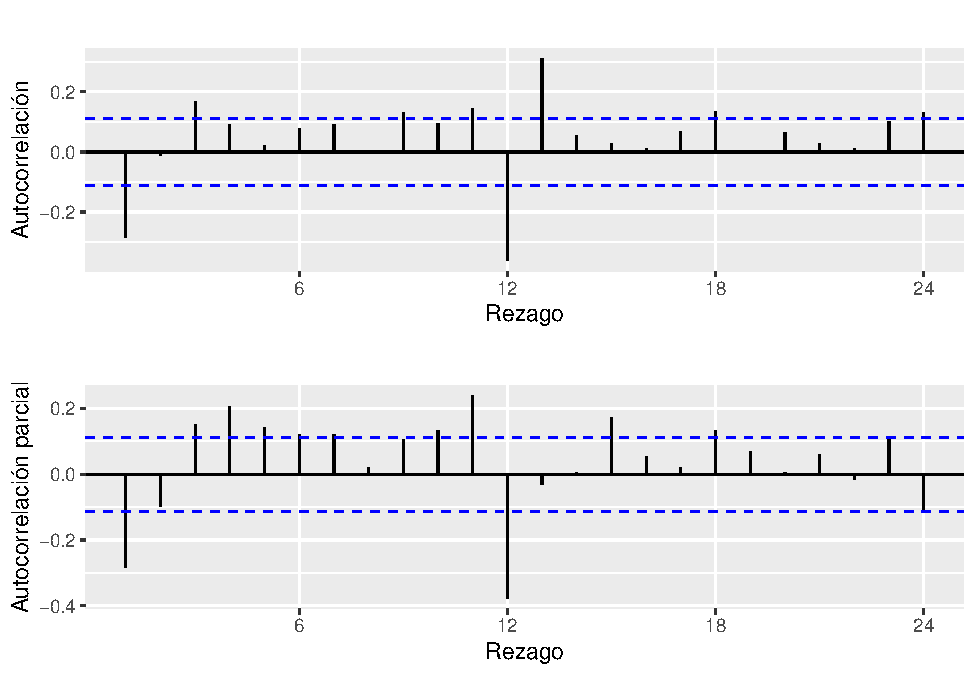
\includegraphics[width=0.75\linewidth]{informe_files/figure-latex/unnamed-chunk-30-1} 

}

\caption{\label{facyp_r1} Funciones de Autocorrelación y Autocorrelación Parcial estimadas de los residuos de un modelo SARIMA(0,0,1)(0,1,1) para el logaritmo del Gasto Público.}\label{fig:unnamed-chunk-30}
\end{figure}

\begin{figure}[H]

{\centering 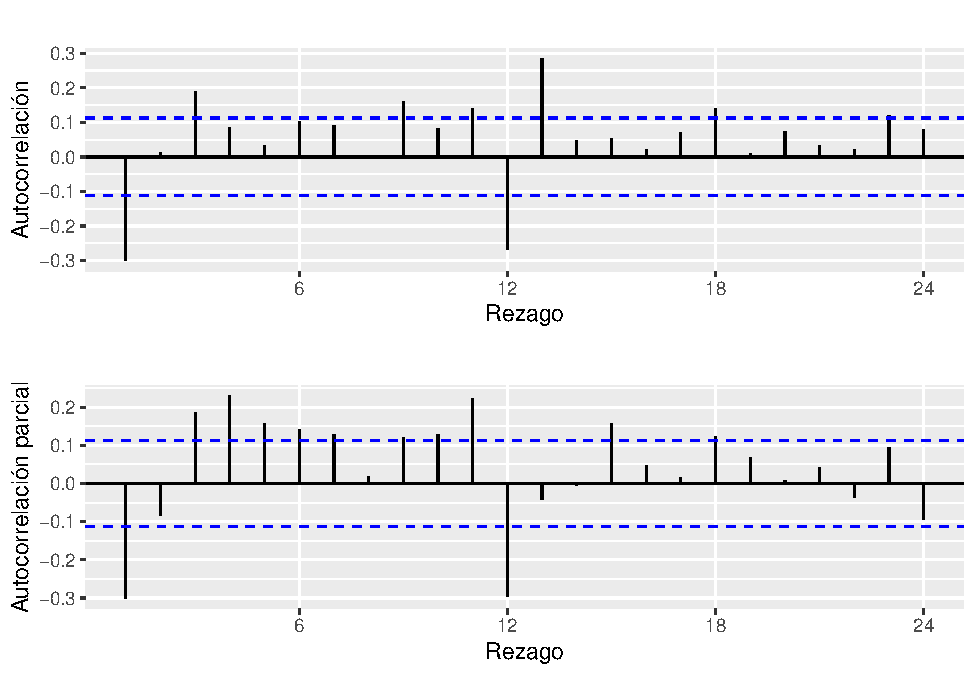
\includegraphics[width=0.75\linewidth]{informe_files/figure-latex/unnamed-chunk-31-1} 

}

\caption{\label{facyp_r2} Funciones de Autocorrelación y Autocorrelación Parcial estimadas de los residuos de un modelo SARIMA(0,0,1)(1,1,0) para el logaritmo del Gasto Público.}\label{fig:unnamed-chunk-31}
\end{figure}

\begin{figure}[H]

{\centering 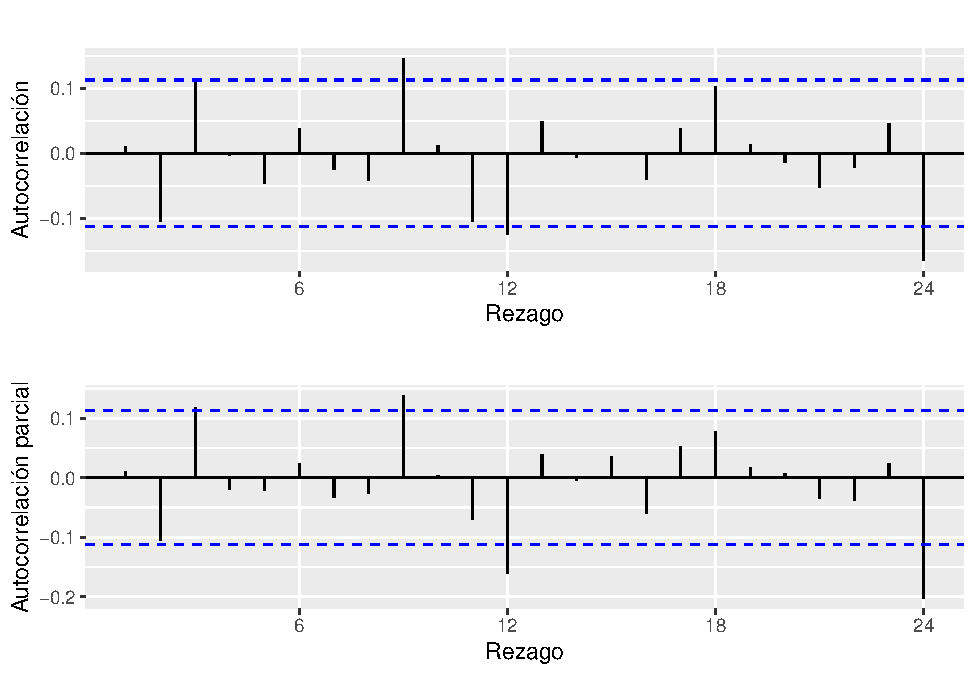
\includegraphics[width=0.75\linewidth]{informe_files/figure-latex/unnamed-chunk-32-1} 

}

\caption{\label{facyp_r3} Funciones de Autocorrelación y Autocorrelación Parcial estimadas de los residuos de un modelo SARIMA(0,1,2)(1,1,0) para el logaritmo del Gasto Público.}\label{fig:unnamed-chunk-32}
\end{figure}

\begin{figure}[H]

{\centering 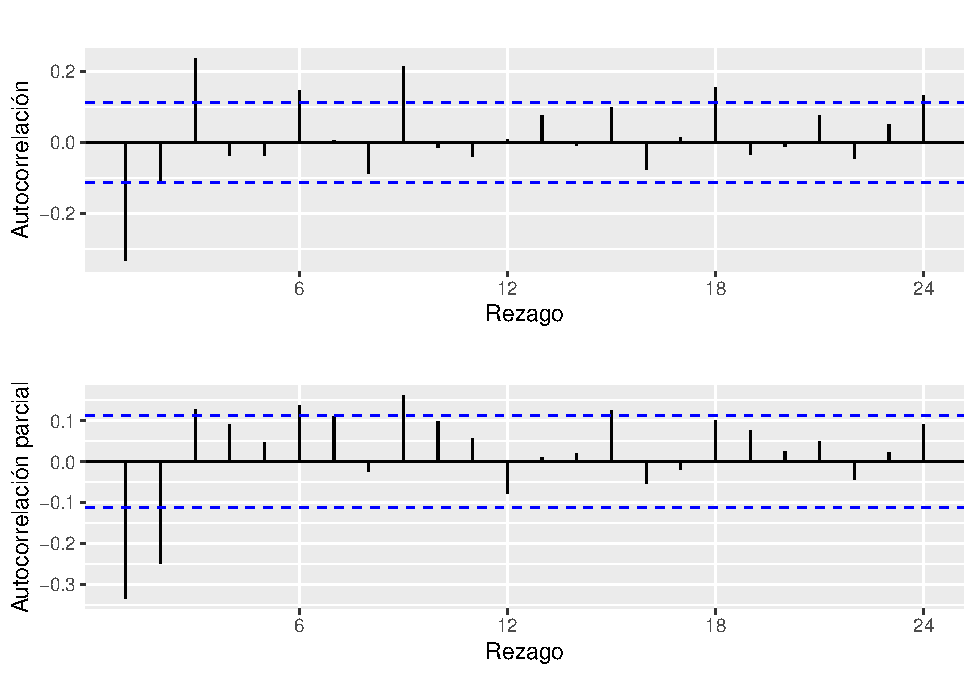
\includegraphics[width=0.75\linewidth]{informe_files/figure-latex/unnamed-chunk-33-1} 

}

\caption{\label{facyp_r4} Funciones de Autocorrelación y Autocorrelación Parcial estimadas de los residuos de un modelo SARIMA(0,1,1)(0,1,1) para el logaritmo del Gasto Público.}\label{fig:unnamed-chunk-33}
\end{figure}

\begin{figure}[H]

{\centering 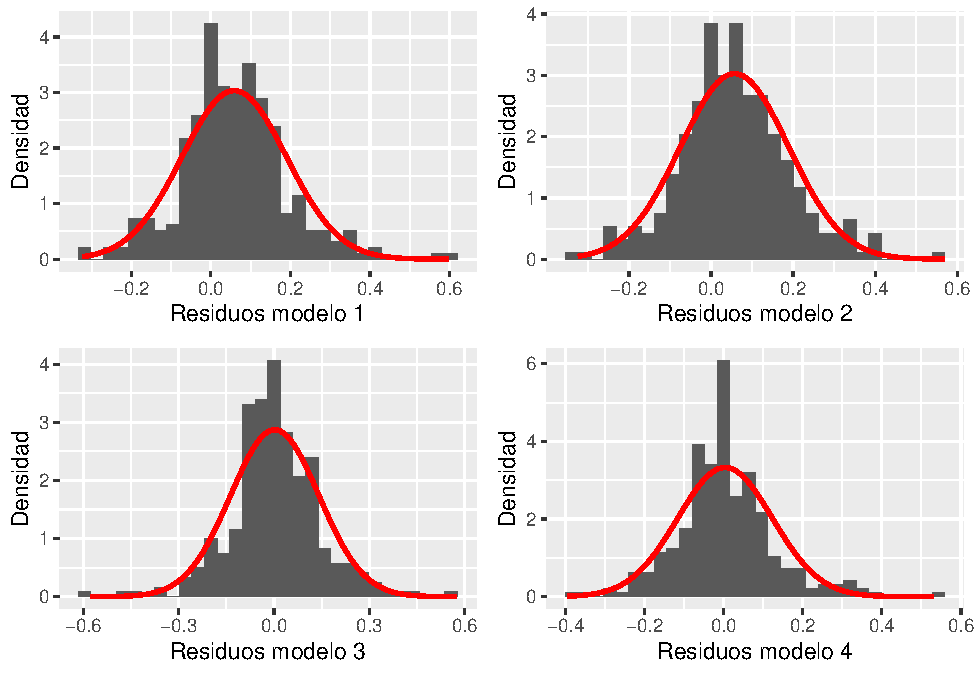
\includegraphics[width=0.75\linewidth]{informe_files/figure-latex/unnamed-chunk-34-1} 

}

\caption{\label{norms} Histograma de los residuos de los modelos reestimados SARIMA intervenido spara el logaritmo del Gasto Público. La línea roja corresponde a una densidad normal con media y desvío muestrales igual al de los residuos.}\label{fig:unnamed-chunk-34}
\end{figure}

\end{document}
